\documentclass[10pt]{beamer}

% theme
\usetheme{PaloAlto}
\usecolortheme{spruce}
\setbeamertemplate{navigation symbols}{}

% packages
\usepackage{hyperref}
\usepackage{graphicx}
\usepackage{caption}
\usepackage{listings}
\usepackage{array}

% caption settings
\captionsetup{font=scriptsize, skip=2pt}

% listings setting
\lstset{
    captionpos=b,
    label={lst:script},
    basicstyle=\tiny\ttfamily,
    keywordstyle=\color{blue},
    commentstyle=\color{green!60!black},
    numbers=left,
    numberstyle=\tiny\color{gray},
    abovecaptionskip=0.8cm
}

% attributes
\title{\textbf{ExaMA WP3 -- Dashboard Performances}}
\author[Tanguy PIERRE]{Tanguy Pierre\\[1cm] \small{Supervisors: V. Chabannes, J. Cladellas}}
\institute{University of Strasbourg}
\date{31th of May}


% **********************  START  **********************
\begin{document}

\frame{\titlepage}


\begin{frame}
    \frametitle{\textbf{Introduction}}

    \begin{itemize}
        \addtolength{\itemsep}{10pt}
        \item Part of the \textit{ExaMA} project from NumPEx 
        \item Benchmarking is for:
        \begin{itemize}
            \item performances comparison
            \item transparency about the evaluation process
            \item references in order to avoid performance decline
            \item data analysis depending on context
        \end{itemize}
    \end{itemize}

    \begin{figure}
        \centering
        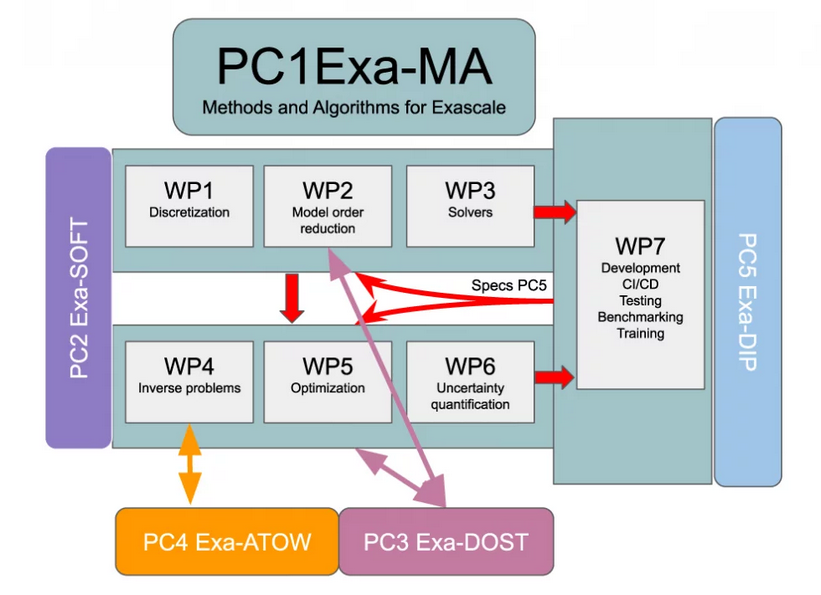
\includegraphics[width=0.6\textwidth]{../illustrations/ExaMa-orga.png}
        \caption{ExaMA organisation}
    \end{figure}
\end{frame}




\begin{frame}
    \frametitle{\textbf{Objectives}}
    \begin{itemize}
        \addtolength{\itemsep}{8pt}
        \item Establish a \textbf{Continuous Integration/Continuous Deployment} workflow. \\
        \item Enhance the \textbf{dashboard presentation} for better visualization of the results. \\
        \item Conducting \textbf{representative tests} is essential to obtain reliable results about the system behaviour. \\
        \item Provide a \textbf{database} for easy access and retrieval of test results. \\
    \end{itemize}

    \begin{figure}
        \centering
        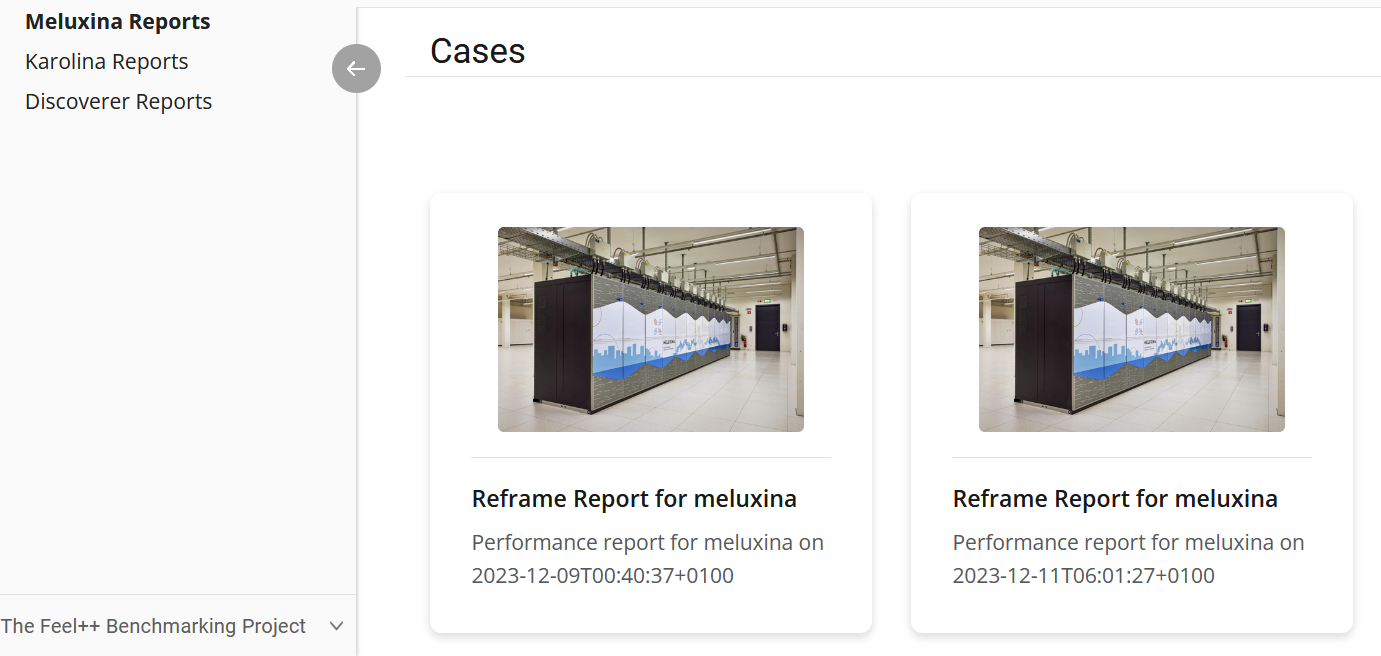
\includegraphics[width=0.6\textwidth]{../illustrations/feelpp-dashboard.png}
        \caption{Feelpp benchmarking platform}
    \end{figure}
\end{frame}

\begin{frame}
    \frametitle{\textbf{Tools}}
    \begin{itemize}
        \addtolength{\itemsep}{7pt}
        \item \textit{ReFrame HPC}, a framework allowing system's complexity abstraction in order to focus only on the algorithm's performance
        \item \textit{Feel++}, a C++ library for Galerkin methods
        \item \textit{Jinja2}, a template engine used for generating the \textit{.adoc}
        \item \textit{Antora}, a documentation site generator \small{(\textit{.adoc} to \textit{.html})}
        \item \textit{Plotly}, the well-known data visualization library
    \end{itemize}

    \begin{figure}
        \centering
        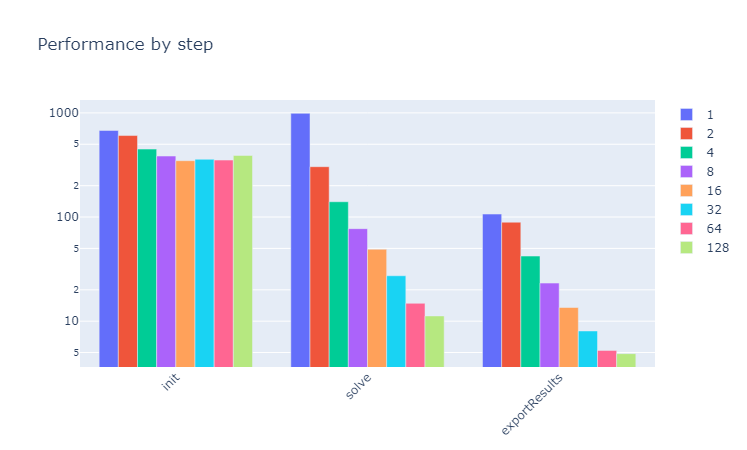
\includegraphics[width=0.6\textwidth]{../illustrations/gaya-graphs/gayaByStep.png}
        \caption{Gaya, Performance by step}
    \end{figure}
\end{frame}


\begin{frame}
    \frametitle{\textbf{Process}}
    \begin{columns}
        \begin{column}{0.5\textwidth}
            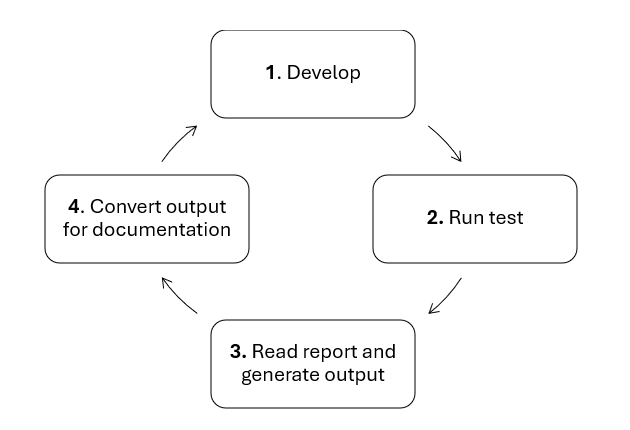
\includegraphics[width=1.1\textwidth]{../illustrations/process.png}
            \captionof{figure}{Gaya, Performance by step}
        \end{column}

        \begin{column}{0.5\textwidth}
            \begin{enumerate}
                \addtolength{\itemsep}{5pt}
                \item Pushing or merging new reports will trigger a new process
                \item Use \textit{ReFrame} for launching multiple tests
                \item \textit{Jinja2} will generate \textit{.adoc} files containing code blocks
                \item \textit{AsciiDoctor} will convert the \textit{.adoc} files into \textit{.html} and Antora will update the documentation site
            \end{enumerate}
        \end{column}
    \end{columns}
\end{frame}

\begin{frame}[fragile]
    \frametitle{\textbf{Process}}
    Here follows the script which controls the launch of the process:
    \vspace{0.5cm}

\begin{lstlisting}[language=bash,caption={Script for process launching}]
rm -rf ~/feelppdb
rm -rf ./build/reframe/output/ ./build/reframe/stage/ ./build/reframe/perflogs

# Variable TO BE SET to the actual HPC
hostname=gaya

current_date=$(date +%Y%m%d)
mkdir -p $(pwd)/docs/modules/${hostname}/pages/reports

export BENCH_CASES_CFG=$(pwd)/src/benchmarking/cases/

# Reframe environment variables
export RFM_CONFIG_FILES=$(pwd)/src/benchmarking/reframe/cluster-config/${hostname}.py
export RFM_REPORT_FILE=$(pwd)/docs/modules/${hostname}/pages/reports/ \
                                            ${hostname}-${current_date}-{sessionid}.json
export RFM_PREFIX=$(pwd)/build/reframe/

reframe -c ./src/feelpp/benchmarking/reframe/regression-tests/heatTest.py \
        -r --system=${hostname} --exec-policy=serial
\end{lstlisting}

\end{frame}

\begin{frame}
    \frametitle{\textbf{Process}}
    \small
    \begin{tabular}{|l|m{8.5cm}|}
        \hline
        \textbf{Line} & \textbf{Description} \\
        \hline
        2-3  & Removing older reports and logs for avoiding unwanted interactions \\
        \hline
        6    & Set up the current machine \\
        \hline
        8    & Get date for reports naming schema \\
        \hline
        9    & Create reports folder if it doesn't already exist \\
        \hline
        11   & Export testcases path \\
        \hline
        14-18   & Export ReFrame environment variables: cluster configuration, report-file with naming schema, output and stage directory\\
        \hline
        20   & Launch Reframe recursevly \textbf{-r} on test defined in the \textit{checkpath} \textbf{-c} with the specified \textit{system}.\\
             & \textbf{--exec-policy=serial} has been set for avoiding some bugs during file access. \\
        \hline
    \end{tabular}
\end{frame}



\end{document}